% !TeX program = xelatex
\documentclass[UTF8,12pt,a4paper]{ctexart}
\usepackage{amsmath,amssymb}
\usepackage{geometry}
\usepackage{tikz} % 引入绘图包以生成几何图形
\geometry{margin=2cm}

% ===== 水印：贺昱琪学习资料 =====
\usepackage{xcolor}
\usepackage{eso-pic}
\usepackage{graphicx}

\newcommand{\WMText}{贺昱琪学习资料}
\newcommand{\WMScale}{2.28}
\newcommand{\WMAngle}{45}
\colorlet{WMColor}{black!8}

\AddToShipoutPictureBG{%
  \AtPageLowerLeft{%
    \put(\LenToUnit{0.66\paperwidth},\LenToUnit{0.70\paperheight}){%
      \rotatebox{\WMAngle}{\scalebox{\WMScale}{\textcolor{WMColor}{\WMText}}}%
    }%
    \put(\LenToUnit{0.33\paperwidth},\LenToUnit{0.50\paperheight}){%
      \rotatebox{\WMAngle}{\scalebox{\WMScale}{\textcolor{WMColor}{\WMText}}}%
    }%
    \put(\LenToUnit{0.66\paperwidth},\LenToUnit{0.30\paperheight}){%
      \rotatebox{\WMAngle}{\scalebox{\WMScale}{\textcolor{WMColor}{\WMText}}}%
    }%
  }%
}

% ===== 5题铺满一页布局 =====
\usepackage{enumitem}
\newcommand{\BottomWriteSpace}{1.5cm}

\newenvironment{OnePageFiveFill}{
  \small
  \vspace*{0pt}
  \begin{enumerate}[leftmargin=*, itemsep=0pt, topsep=0pt, parsep=0pt, partopsep=0pt]
  \setlength{\parskip}{0pt}
}{
  \end{enumerate}
  \vspace*{\BottomWriteSpace}
  \normalsize
  \newpage
}

\newcommand{\Q}[1]{\item #1\par\vfill}
\newcommand{\Qlast}[1]{\item #1\par}

\begin{document}

% =========================================================
% 5.25
% =========================================================
\section*{5月25日作业（5道题当晚22:00前打卡）}
\begin{OnePageFiveFill}

\Q{计算：$\displaystyle \frac{2025 + \dfrac{1}{2024}}{2024 + \dfrac{1}{2025}} - \frac{2023 + \dfrac{1}{2024}}{2024 + \dfrac{1}{2023}}$}

\Q{一辆汽车从甲地开往乙地。如果减速 $\dfrac{1}{10}$，则要比原定时间迟到 1 小时；如果以原速行驶 180 千米，再提速 $\dfrac{1}{5}$，则可比原定时间早到 1 小时。甲、乙两地的距离是多少千米？}

\Q{
\begin{minipage}[c]{0.75\textwidth}
如图，圆中三个小正方形（涂色部分）A, B, C 的边长分别是 2 厘米、3 厘米、4 厘米，则最大正方形的面积是\underline{\hspace{3em}}平方厘米，圆的面积是\underline{\hspace{3em}}平方厘米。（$\pi$ 取 3.14）
\end{minipage}
\hfill
\begin{minipage}[c]{0.2\textwidth}
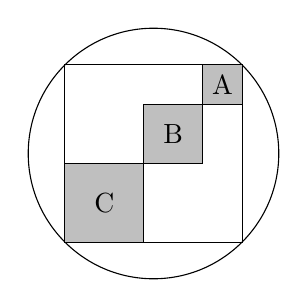
\begin{tikzpicture}[scale=0.25]
\draw (4.5, 4.5) circle (6.364);
\draw (0,0) rectangle (9,9);
\filldraw[fill=black!25, draw=black] (0,0) rectangle (4,4) node[midway] {C};
\filldraw[fill=black!25, draw=black] (4,4) rectangle (7,7) node[midway] {B};
\filldraw[fill=black!25, draw=black] (7,7) rectangle (9,9) node[midway] {A};
\end{tikzpicture}
\end{minipage}
}

\Q{（在环形跑道上，小明和小华同时从同一地点同向而行，每隔 30 分钟小明就可以追上小华一次。若两人在原地同时出发，相背而行，则每隔 10 分钟就相遇一次。两人跑一圈各需几分钟？}

\Qlast{解方程：$\dfrac{3x+1}{2} - \dfrac{2x-3}{3} = \dfrac{x+5}{6}$}

\end{OnePageFiveFill}

% =========================================================
% 5.26
% =========================================================
\section*{5月26日作业（5道题当晚22:00前打卡）}
\begin{OnePageFiveFill}

\Q{计算：$\displaystyle \frac{100 + \dfrac{1}{99}}{99 + \dfrac{1}{100}} - \frac{98 + \dfrac{1}{99}}{99 + \dfrac{1}{98}}$}

\Q{一辆汽车从甲地开往乙地。如果减速 $\dfrac{1}{5}$，则要比原定时间迟到 1 小时；如果以原速行驶 120 千米，再提速 $\dfrac{1}{3}$，则可比原定时间早到 0.5 小时。甲、乙两地的距离是多少千米？}

\Q{
\begin{minipage}[c]{0.75\textwidth}
如图，圆中三个小正方形（涂色部分）A, B, C 的边长分别是 1 厘米、2 厘米、3 厘米，则最大正方形的面积是\underline{\hspace{3em}}平方厘米，圆的面积是\underline{\hspace{3em}}平方厘米。（$\pi$ 取 3.14）
\end{minipage}
\hfill
\begin{minipage}[c]{0.2\textwidth}
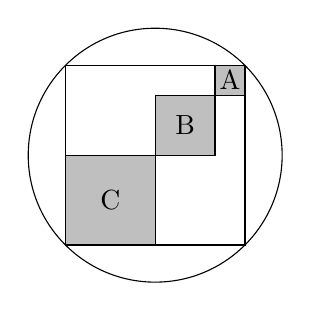
\begin{tikzpicture}[scale=0.38]
\draw (3, 3) circle (4.243);
\draw (0,0) rectangle (6,6);
\filldraw[fill=black!25, draw=black] (0,0) rectangle (3,3) node[midway] {C};
\filldraw[fill=black!25, draw=black] (3,3) rectangle (5,5) node[midway] {B};
\filldraw[fill=black!25, draw=black] (5,5) rectangle (6,6) node[midway] {A};
\end{tikzpicture}
\end{minipage}
}

\Q{在环形跑道上，小明和小华同时从同一地点同向而行，每隔 12 分钟小明就可以追上小华一次。若两人在原地同时出发，相背而行，则每隔 4 分钟就相遇一次。两人跑一圈各需几分钟？}

\Qlast{解方程：$\dfrac{4x+3}{3} - \dfrac{3x-1}{2} = \dfrac{x+5}{6}$}

\end{OnePageFiveFill}

% =========================================================
% 5.27
% =========================================================
\section*{5月27日作业（5道题当晚22:00前打卡）}
\begin{OnePageFiveFill}

\Q{计算：$\displaystyle \frac{50 + \dfrac{1}{49}}{49 + \dfrac{1}{50}} - \frac{48 + \dfrac{1}{49}}{49 + \dfrac{1}{48}}$}

\Q{（分数的应用）一辆汽车从甲地开往乙地。如果减速 $\dfrac{1}{6}$，则要比原定时间迟到 1 小时；如果以原速行驶 160 千米，再提速 $\dfrac{1}{4}$，则可比原定时间早到 0.6 小时。甲、乙两地的距离是多少千米？}

\Q{
\begin{minipage}[c]{0.75\textwidth}
（面积计算技巧）如图，圆中三个小正方形（涂色部分）A, B, C 的边长分别是 2 厘米、4 厘米、6 厘米，则最大正方形的面积是\underline{\hspace{3em}}平方厘米，圆的面积是\underline{\hspace{3em}}平方厘米。（$\pi$ 取 3.14）
\end{minipage}
\hfill
\begin{minipage}[c]{0.2\textwidth}
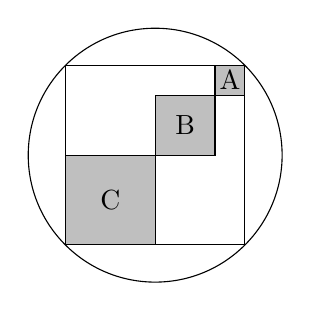
\begin{tikzpicture}[scale=0.19]
\draw (6, 6) circle (8.485);
\draw (0,0) rectangle (12,12);
\filldraw[fill=black!25, draw=black] (0,0) rectangle (6,6) node[midway] {C};
\filldraw[fill=black!25, draw=black] (6,6) rectangle (10,10) node[midway] {B};
\filldraw[fill=black!25, draw=black] (10,10) rectangle (12,12) node[midway] {A};
\end{tikzpicture}
\end{minipage}
}

\Q{（相遇问题）在环形跑道上，小明和小华同时从同一地点同向而行，每隔 24 分钟小明就可以追上小华一次。若两人在原地同时出发，相背而行，则每隔 8 分钟就相遇一次。两人跑一圈各需几分钟？}

\Qlast{解方程：$\dfrac{5x-1}{6} - \dfrac{2x+3}{4} = \dfrac{x-3}{2}$}

\end{OnePageFiveFill}

% =========================================================
% 5.28
% =========================================================
\section*{5月28日作业（5道题当晚22:00前打卡）}
\begin{OnePageFiveFill}

\Q{计算：$\displaystyle \frac{202 + \dfrac{1}{201}}{201 + \dfrac{1}{202}} - \frac{200 + \dfrac{1}{201}}{201 + \dfrac{1}{200}}$}

\Q{一辆汽车从甲地开往乙地。如果减速 $\dfrac{1}{8}$，则要比原定时间迟到 1 小时；如果以原速行驶 210 千米，再提速 $\dfrac{1}{6}$，则可比原定时间早到 0.5 小时。甲、乙两地的距离是多少千米？}

\Q{
\begin{minipage}[c]{0.75\textwidth}
如图，圆中三个小正方形（涂色部分）A, B, C 的边长分别是 3 厘米、4 厘米、5 厘米，则最大正方形的面积是\underline{\hspace{3em}}平方厘米，圆的面积是\underline{\hspace{3em}}平方厘米。（$\pi$ 取 3.14）
\end{minipage}
\hfill
\begin{minipage}[c]{0.2\textwidth}
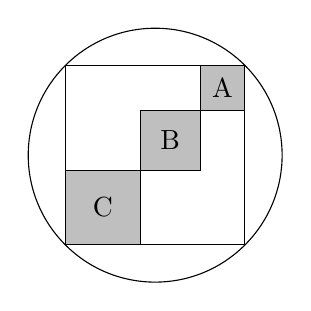
\begin{tikzpicture}[scale=0.19]
\draw (6, 6) circle (8.485);
\draw (0,0) rectangle (12,12);
\filldraw[fill=black!25, draw=black] (0,0) rectangle (5,5) node[midway] {C};
\filldraw[fill=black!25, draw=black] (5,5) rectangle (9,9) node[midway] {B};
\filldraw[fill=black!25, draw=black] (9,9) rectangle (12,12) node[midway] {A};
\end{tikzpicture}
\end{minipage}
}

\Q{在环形跑道上，小明和小华同时从同一地点同向而行，每隔 60 分钟小明就可以追上小华一次。若两人在原地同时出发，相背而行，则每隔 12 分钟就相遇一次。两人跑一圈各需几分钟？}

\Qlast{解含小数的方程：$\dfrac{1.6x - 0.8}{0.4} - \dfrac{1.2x + 3}{0.6} = 5$}

\end{OnePageFiveFill}

% =========================================================
% 5.29
% =========================================================
\section*{5月29日作业（5道题当晚22:00前打卡）}
\begin{OnePageFiveFill}

\Q{计算：$\displaystyle \frac{30 + \dfrac{1}{29}}{29 + \dfrac{1}{30}} - \frac{28 + \dfrac{1}{29}}{29 + \dfrac{1}{28}}$}

\Q{一辆汽车从甲地开往乙地。如果减速 $\dfrac{1}{4}$，则要比原定时间迟到 2 小时；如果以原速行驶 240 千米，再提速 $\dfrac{1}{2}$，则可比原定时间早到 1 小时。甲、乙两地的距离是多少千米？}

\Q{
\begin{minipage}[c]{0.75\textwidth}
（面积计算技巧）如图，圆中三个小正方形（涂色部分）A, B, C 的边长分别是 1 厘米、3 厘米、4 厘米，则最大正方形的面积是\underline{\hspace{3em}}平方厘米，圆的面积是\underline{\hspace{3em}}平方厘米。（$\pi$ 取 3.14）
\end{minipage}
\hfill
\begin{minipage}[c]{0.2\textwidth}
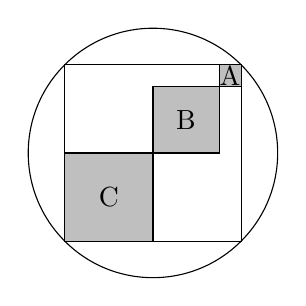
\begin{tikzpicture}[scale=0.28]
\draw (4, 4) circle (5.657);
\draw (0,0) rectangle (8,8);
\filldraw[fill=black!25, draw=black] (0,0) rectangle (4,4) node[midway] {C};
\filldraw[fill=black!25, draw=black] (4,4) rectangle (7,7) node[midway] {B};
\filldraw[fill=black!25, draw=black] (7,7) rectangle (8,8) node[midway] {A};
\end{tikzpicture}
\end{minipage}
}

\Q{（相遇问题）在环形跑道上，小明和小华同时从同一地点同向而行，每隔 15 分钟小明就可以追上小华一次。若两人在原地同时出发，相背而行，则每隔 5 分钟就相遇一次。两人跑一圈各需几分钟？}

\Qlast{$\dfrac{1.5x - 0.5}{0.5} - \dfrac{2x + 1}{0.2} = -2$}

\end{OnePageFiveFill}

\end{document}